%\documentclass[article,pdftex,10pt,a4paper,twocolumn]{article}
\documentclass[article,pdftex,12pt,a4paper]{article}
\usepackage[authoryear]{natbib}
\usepackage{graphics}

\usepackage{url}\urlstyle{rm}
\usepackage{epstopdf}
\usepackage{graphicx}

\RequirePackage{color}
\def\imagei{\centerline{\color[gray]{.75}\rule{\hsize}{4pc}}}%
\def\imageii{\centerline{\color[gray]{.75}\rule{4pc}{4pc}}}%


\begin{document}


\title{Analysis of Indie EDM since 2010}

\author{Jacob Bengel \\ \small Kansas State University, Manhattan, KS 66502 \\ \small jbengel@ksu.edu}

\date{December 11, 2024}

\maketitle

\begin{abstract}
The abstract is a single paragraph of 150-300 words, which summarizes your project, and can be read independently of the rest of the paper. The abstract should define the scope of the research project, the methods that were used, and the results and conclusions. It should also summarize the key discoveries. TODO Lorem ipsum odor amet, consectetuer adipiscing elit. Vestibulum etiam sagittis phasellus auctor senectus nullam duis. Orci netus tortor montes fames feugiat nibh urna. Senectus eleifend blandit fusce sit sodales neque quam. Efficitur blandit montes commodo elit euismod platea justo. Lacinia in class hendrerit fusce dis fermentum dictum mattis. Leo pretium ullamcorper ultrices arcu ex risus sit potenti. Suscipit laoreet hendrerit; conubia gravida tristique nulla commodo pulvinar. Turpis curabitur porta et pharetra habitant etiam nam. Sociosqu ultricies risus habitasse convallis vitae? Penatibus aliquet potenti commodo aliquet laoreet; mollis molestie suscipit pharetra. Curabitur lectus velit quis, laoreet hendrerit est nisi tortor. Venenatis congue lobortis proin tempus ante ornare magna ad. Magnis conubia class tempor himenaeos lacinia libero. Taciti sem fermentum morbi penatibus hac sodales sed? Nec primis venenatis facilisis interdum faucibus sollicitudin nulla? Finibus viverra nec quisque facilisis eget ultrices neque in. Accumsan eu ultrices aliquam sagittis accumsan. Nibh pharetra cubilia sit ut lacus penatibus quam et. Metus auctor nec nec a leo dolor proin. Inceptos erat tempor aptent mus faucibus ornare fames venenatis. Ultrices vitae posuere felis felis nostra pharetra sem. Habitasse sem dignissim torquent est mus vivamus massa eu tristique. Facilisi sem hac aliquet aptent dui sodales sollicitudin. Blandit aliquam dictum natoque rutrum quisque. Etiam a ridiculus eu; vulputate.
\end{abstract}



\section{Introduction}
%\label{synopsis}
% The introduction section should include the following:
% a. Description of the problem that is being addressed, and an explanation of why
% the problem is difficult and why it is important to solve it.
% b. A summary of previous work that was done for solving the problem at hand. This
% should include references to papers published previously that described solutions to
% the same or similar problems. These papers should also be listed in the
% Bibliography section.
As done by \cite{einstein2013einstein} and \cite{dhar2013data}.

The introduction section should provide a brief description of the project, and a summary of the data, and a summary of the primary insights that were made during the project.

References should be used with the APA format. That can be done easily by using Bibtex with the apalike bibliography style. A reference to a bibliographic source in the text can be done using \cite{ozsvath2001approaches} or \citep{ellis1979homogeneity}.

If the name of the author of the paper is part of the sentence, the reference should be: \cite{ozsvath2001approaches} proposed a different cosmological model based on a rotating universe. 

If the name of the author is not part of the sentence, the reference should be. In addition to the standard cosmological models, alternative cosmological models were proposed \citep{ozsvath2001approaches}.

A reference to more than one source can be done by \citep{ozsvath1962finite,godel1949example}.

The introduction section is a mandatory section that all reports must include. The rest of the report, except for the {\it Data} section, can include different sections.


\section{"Methods"}
%\label{data}
(Data) In this section you need to describe your data. The description should include the files, formats, size of the data (number of columns, rows in each file) and a description of each column/field. Each column should be described by specifying the data type and the distribution of the values. Visualization is also expected in the form of tables and/or figures. A simple table can be formatted as follows:

\begin{table}[h]
{
%\footnotesize
\scriptsize
\begin{tabular}{|l|c|c|c|c|}
\hline
Column 1 &  Column 2    &  Column 3  & Column 4 & Column 5 \\      
\hline
0   &    9,655   &   64,092  &  10,862     &    84,609    \\
0.05 &   14,746  &  104,339   & 21,098   &   140,183    \\
0.1 &    12,142  &  67,712  &  13,797   &    93,651    \\   
0.15  &  7,757    & 33,957  &  8,360     &     50,074    \\
$>$0.2  &  47,456    & 134,706    & 36,473    &   218,635    \\
\hline
Total      &  91,965 &  406,185  & 90,899   & 589,049  \\
\hline        
\end{tabular}
\caption{Each table must have a caption.}
\label{table_label}

}
\end{table}

A simple figure can be formatted using the following syntax. You can use several image formats such as eps or jpeg, but pdf is preferred.

\begin{figure*}
\centering
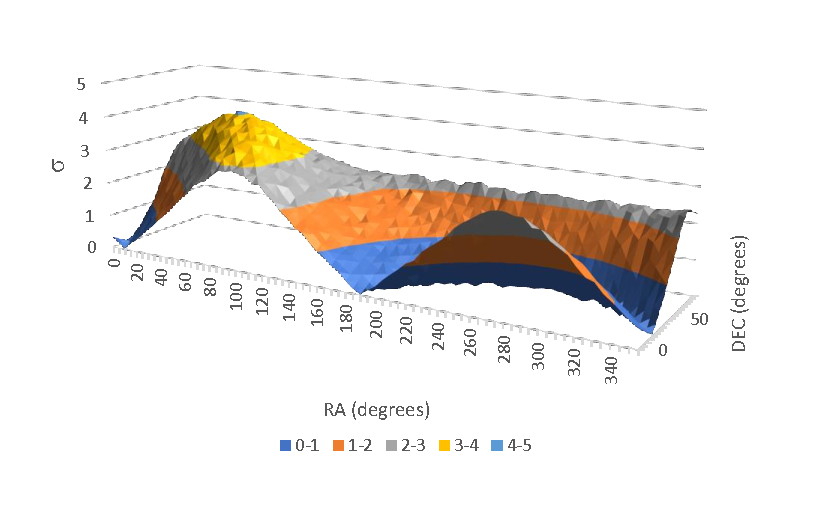
\includegraphics[scale=1.0]{figure_file.pdf}
\caption{Each figure must have a caption}
\label{figure_label}
\end{figure*}

Any rendering or wrangling of the data should also be described.



\section{"Results"}
%\label{method}
(Supervised ML blahblahblah) The rest of the sections should describe the data science tools and paradigms used, and the results and insights they led to. 

This section should describe in details the methods that you developed and/or used. A method can be a certain existing software tool that you used, an equation, an algorithm, etc’.  If you used existing methods, a reference to the papers that describe the methods is required.

The insights described in the report are also the same insights described in the abstract and synopsis, but with far more details.



\section{Conclusion}
%\label{conclusion}
In this section you can provide a short summary of the conclusion of the work, and what you can conclude from your experience working on the data. That can include suggestions of improving the data, ideas to improve the analysis, or opportunities for future work and things that can be done in the future.

It should also discuss the weaknesses of the analysis, and things we cannot conclude from our results. You can also use the Conclusion section to discuss potential other uses of the work.



\section*{Acknowledgments}
Dr. Lior Shamir for a job well done teaching Data Science Foundations during the Fall 2024 semester and providing references on Essentia and LaTeX use.



\bibliography{main}
\bibliographystyle{apalike}



\end{document}



